\chapter{Reti Bayesiane} \label{cap:RetiBayesiane}
\section{Introduzione}
Le reti bayesiane sono un \textbf{modello grafico probabilistico} che rappresenta
le relazioni probabilistiche tra un insieme di variabili. Queste reti sono utili
per rappresentare le relazioni di dipendenza tra le variabili e per effettuare
inferenze su di esse. Le dipendenze espresse graficamente dalle reti Bayesiane
sono solo assunzioni sul dominio, dal momento che vengono stimate usando algoritmi
o usando l'esperienza delle persone afferenti al dominio.

Usando l'indipendenza e l'indipendenza condizionata il modello causale è molto
più compatto, il numero di parametri utilizzato si riduce.
\begin{definizione}[\textbf{Rete Bayesiana}]
    Una \textbf{rete Bayesiana} è un \textbf{grafo orientato aciclico} in cui i
    nodi sono annotati con una \textbf{informazione quantitativa}, ovvero la
    tabella di probabilità condizionata (CPT), e gli archi definiscono la
    \textbf{dipendenza e indipendenza condizionale} tra le variabili rappresentate
    dai nodi.
\end{definizione}
\begin{nota}
    Le variabili rappresentate dai nodi possono essere continue o discrete.
\end{nota}
Di norma diremo che se esiste l'arco $(x,y)\in E$ allora $x$ causa $y$, in altri
termini $x$ è genitore di $y$ o $y$ è figlio di $x$.
\begin{center}
    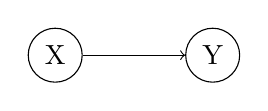
\begin{tikzpicture}
        \node[shape=circle,draw=black] (X) at (0,0) {X};
        \node[shape=circle,draw=black] (Y) at (2,0) {Y};
        \path [->] (X) edge node {} (Y);
    \end{tikzpicture}
\end{center}
\begin{definizione}[\textbf{Condizionalmente indipendente}]
    L'evento $A$ è \textbf{condizionalmente indipendente} dall'evento $B$, se dato
    un evento $C$ vale la seguente relazione:
    \begin{equation}
        P(A|B,C) = P(A|C)
    \end{equation}
    ovvero che la conoscenza a priori di $B$ non influisce sulla probabilità di
    $A$ rispetto a quella che si ha conoscendo $C$.
\end{definizione}
La topologia della rete, ovvero la sua struttura, e le probabilità condizionate
dei nodi dati i loro genitori sono sufficienti a specificare la \textbf{distribuzione
    congiunta} di tutte le variabili rappresentate dalla rete.

La componente quantitativa contenuta in ogni nodo è costituita da un insieme di
\textbf{tabelle di probabilità condizionate} (CPT), queste tabelle rappresentano
l'impatto dei genitori sulla variabile stessa.

Le CPT dicono quant'è la probabilità di assumere un valore per una variabile di
un nodo, condizionata al valore delle variabili dei genitori. L'\textbf{assunzione}
delle reti è che ogni nodo è \textbf{condizionalmente indipendente} dai suoi non
discendenti dati i suoi genitori.

Nella definizione della struttura della rete è importante che il grafo orientato
non contenga cicli, ovvero che la rete Bayesiane sia un DAG (\textit{Directed Acyclic
    Graph}). Questo perché non è possibile che una variabile sia causa di se stessa.
\subsection{Componente Quantitativa}
Consideriamo ora la componente quantitativa di una rete Bayesiane, ovvero le
\textbf{Conditional Probability Tables} (CPT). Di queste tabelle possiamo dire che:
\begin{itemize}
    \item Ogni nodo ha associata una tabella (CPT).
    \item La CPT descrive la probabilità condizionata della variabile dato un
          particolare assegnamento dei valori delle variabili genitore.
    \item La somma di ogni riga della tabella deve essere uguale a $1$.
    \item La CPT di una variabile booleana con $k$ variabili genitori anche essi
          booleani, contiene $2^k$ valori di probabilità che possono essere
          specificati indipendentemente.
    \item Una variabile senza genitori ha una CPT con una sola riga che contiene
          i valori di probabilità a priori per ogni possibile valore che la
          variabile può assumere.
\end{itemize}
\begin{nota}
    Nel caso specifico di variabili booleane, se specifico solo il valore nel
    caso vero nella CPT posso ricavare il valore del caso falso utilizzando:
    \begin{equation*}
        \text{falso} = 1 - \text{vero}
    \end{equation*}
    Quindi il falso è un parametro dipendente.
\end{nota}
Per le reti Bayesiane si può fare sia inferenza \textit{diagnostica}, ovvero fatta
dai figli verso i genitori, sia \textit{prognostica} dai genitori verso i figli.
Posso anche calcolare la probabilità di variabili che non sono in relazione padre
figlio ma che sono connesse.
\section{Semantica delle reti Bayesiane}
La semantica delle reti Bayesiane può essere presentata e compresa in base a:
\begin{itemize}
    \item \textbf{Semantica numerica}: la rete rappresenta una \textbf{distribuzione
              congiunta} di probabilità. Questa invece risulta importante per
          comprendere come sia possibile effettuare inferenza utilizzando la
          probabilità congiunta.
    \item \textbf{Semantica topologica}: la rete codifica un insieme di
          \textbf{relazioni di indipendenza condizionale}. Questa risulta
          importante per comprendere come sia possibile costruire un modello di
          Rete Bayesiane.
\end{itemize}
La costruzione delle reti è un processo incrementale che può essere effettuato
utilizzando le informazioni a priori del dominio se si hanno conoscenze
approfondite di esso, oppure tramite algoritmi di apprendimento.
\subsection{Semantica numerica}
Ogni rete costituisce una descrizione completa del dominio che rappresenta, di
conseguenza la distribuzione congiunta di probabilità di tutte le variabili
rappresentate dalla rete può essere ottenuta direttamente dalla rete stessa.

Un generico elemento della distribuzione di probabilità congiunta è associato a
una realizzazione congiunta delle variabili presenti nella rete.

Ogni elemento della distribuzione di probabilità congiunta può essere calcolato
sfruttando la \textbf{formula di fattorizzazione della distribuzione congiunta}
che è data da:
\begin{equation}
    P(V_1 = v_1,...,V_n = v_n) = \prod_{i=1}^{n} P(V_i=v_i|parents(V_i))
\end{equation}
dove $parents(V_i)$ rappresenta la realizzazione congiunta dei genitori di $V_i$.
Ogni elemento della distribuzione congiunta è rappresentato tramite il prodotto
delle opportune componenti delle CPT dei nodi della rete.
\begin{nota}
    Ricorda che per il teorema di Bayes:
    \begin{equation*}
        P(V_i = v_i|parents(V_i)) = \frac{P(V_i = v_i,parents(V_i))}{P(parents(V_i))}
        = \alpha P(V_i = v_i,parents(V_i))
    \end{equation*}
    Quindi la probabilità condizionata viene considerata come la probabilità
    congiunta divisa per la probabilità degli eventi congiunti. Per semplificare
    la probabilità si può solo calcolare la congiunta e successivamente moltiplicarla
    per il fattore $\alpha$ di normalizzazione.

    Il valore di $\alpha$ per la probabilità $P(V_i=v_i|parents(V_i))$ si trova
    nel seguente modo:
    \begin{equation*}
        \alpha = \frac{1}{P(V_i = \lnot v_i, parents(V_i)) + P(V_i = v_i,parents(V_i))}
    \end{equation*}
\end{nota}
\begin{nota}
    Non si vedono più le dipendenze di una variabile da tutte le altre ma bensì
    probabilità della variabile condizionata dai suoi genitori.
\end{nota}
\subsection{Semantica topologica}
La formula di fattorizzazione implica relazioni di \textbf{indipendenza condizionale}
che possono essere sfruttate per determinare la componente \textbf{topologica}
della rete.

La regola della probabilità congiunta la possiamo scrivere come:
\begin{equation*}
    \begin{aligned}
        P(V_1= v_1,...,V_n = v_n) = P(V_1 = v_1) \cdot P(V_2 = v_2|V_1 = v_1)
        \cdot P(V_3 = v_3|V_1 = v_1,V_2 = v_2) \dots \\
        \dots P(V_n = v_n|V_1 = v_1, \dots,V_{n-1}=v_{n-1}) = \prod_{i=1}^{n}
        P(V_i = v_i| \bigcap_{j = 1}^{i - 1} V_j= v_j)
    \end{aligned}
\end{equation*}
Questa uguaglianza è vera per ogni insieme di variabili aleatorie ed è nota con
il nome di \textbf{chain rule}. Confrontando la formula di fattorizzazione con
la chain rule è possibile verificare che la specificazione della distribuzione
di probabilità congiunta è equivalente all'asserzione generale che per ogni
variabile $v_i$:
\begin{equation}
    P(v_i|v_1,...,v_{i-1}) = P(v_i|parents(v_i))
\end{equation}
a patto che $parents(v_i) \subseteq \{v_1,...,v_{i-1}\}$. Quindi possiamo
considerare la probabilità di $V_i$ condizionata da tutti gli altri nodi della
rete, può essere vista come la probabilità di $V_i$ condizionata solamente dai
suoi genitori. Questo ci permette di effettuare una semplificazione molto utile.

Una rete Bayesiane rappresenta correttamente un dominio solo a condizione che ogni
nodo risulti \textbf{condizionalmente indipendente} dai suoi non discendenti
dati i suoi genitori. Pertanto, per costruire una Rete Bayesiana che abbia la
corretta struttura del dominio da modellare è necessario scegliere, per ogni nodo,
i nodi genitore in modo che tale proprietà risulti verificata. In aggiunta un nodo
è \textbf{condizionalmente indipendente} da tutti i nodi restanti della rete data
la conoscenza dello stato del suo \textbf{Markov Blanket}, ovvero l'insieme dei
genitori, dei figli e dei genitori dei figli.
\begin{figure}[!ht]
    \centering
    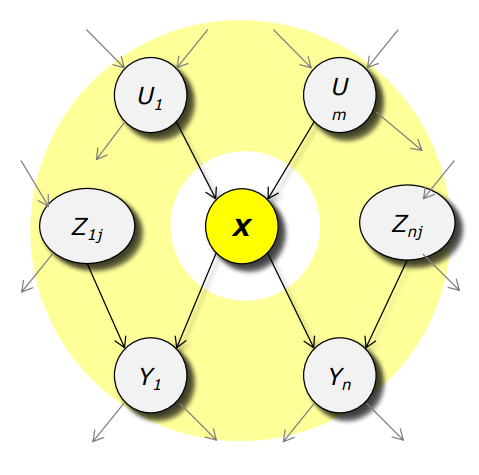
\includegraphics[width=0.35\textwidth]{./img/Reti/MarkovBlanket.png}
    \caption{I nodi $U_i, Z_{ij}, Y_j$ appartengono alla Markov Blanket di $X$}
    \label{fig:MarkovBlanket}
\end{figure}

Una possibile procedura per la costruzione incrementale della componente topologica
di una rete Bayesiane è la seguente:
\begin{itemize}
    \item Scegliere un insieme di variabili $\{x_1, \dots, x_n\}$ che rappresentano
          le variabili del dominio.
    \item Scegliere un ordinamento topologico per le variabili.
    \item Inizializzare il numero dei nodi aggiunti alla rete a $i = 1$.
    \item Selezionare la variabile $X_i$ e aggiungere il nodo corrispondente alla
          rete.
          \begin{itemize}
              \item Porre $parents(X_i)$ uguale all'insieme minimale di nodi,
                    appartenenti alla rete nel momento corrente $\{X_{(1)} \dots X_{(i-1)}\}$
                    che soddisfa la proprietà di indipendenza condizionale.
              \item Computare la CPT per la variabile $X_i$.
          \end{itemize}
    \item Incrementare il numero dei nodi aggiunti alla rete $i=i+1$. E ripetere il
          procedimento per ogni variabile.
\end{itemize}
Il metodo di costruzione delle reti è un passo fondamentale per la corretta
rappresentazione del dominio. La scelta delle relazioni di dipendenza condizionale
impatta notevolmente sulla quantità di parametri che devono essere specificati
per la rete.

Oltre a costituire una rappresentazione completa e non ridondante di un dominio
una Rete Bayesiane è spesso molto più compatta dell'intera distribuzione di
probabilità congiunta. Questo rende possibile il trattamento di domini
caratterizzati da un numero molto elevato di variabili.

La compattezza delle Reti Bayesiane è un esempio della proprietà dei sistemi
strutturati localmente o sparsi. In ogni sistema strutturato localmente ogni
sotto-componente interagisce solo con un numero limitato di altre componenti,
indipendentemente dal numero totale di componenti del sistema.

La strutturazione locale è di norma associata ad un fattore di crescita della
complessità lineare e non esponenziale. Nel caso di una Rete Bayesiana è
ragionevole ipotizzare che ogni variabile sia direttamente influenzata da al
massimo $k$ variabili.

Nel caso in cui si consideri una Rete Bayesiane costituita da $n$ variabili
Booleane avremo che la quantità di informazione necessaria per specificare una
qualsiasi CPT è limitata superiormente da $2^k$ numeri per cui la rete completa
richiede di specificare al più $n \cdot 2^k$ numeri. Mentre specificare l'intera
distribuzione congiunta di probabilità richiede $2^n$ numeri.
\subsection{Indipendenza condizionata}
Esiste un metodo per scoprire se in una rete Bayesiana due variabili sono
condizionalmente indipendenti. Questo metodo prende il nome di \textbf{D-separazione}.
\begin{definizione}[\textbf{D-separazione}]
    Due nodi $X$ e $Z$ sono \textbf{D-separati} da un insieme $E$ di variabili con
    evidenza se e solo se ogni cammino non orientato da $X$ a $Z$ è \textbf{bloccato}.
\end{definizione}
\begin{definizione}[\textbf{cammino bloccato}]
    Un cammino è \textbf{bloccato} se e solo se vale almeno una delle seguenti
    condizioni:
    \begin{itemize}
        \item Se esiste una variabile $V$ tale che appartiene alle evidenze e
              gli archi del camino sono \textbf{tail-to-tail}.
              \begin{figure}[!ht]
                  \centering
                  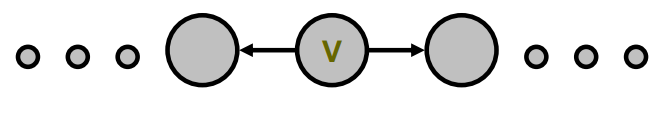
\includegraphics[width=0.35\textwidth]{./img/Reti/TailToTail.png}
                  \caption{Collegamento tail-to-tail}
                  \label{fig:tail-to-tail}
              \end{figure}
        \item Se esiste una variabile $V$ tale che appartiene alle evidenze e
              gli archi che collegano $V$ sono \textbf{tail-to-head}.
              \begin{figure}[!ht]
                  \centering
                  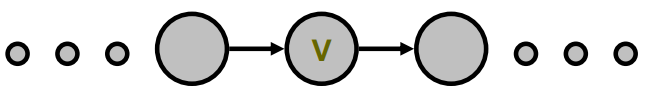
\includegraphics[width=0.35\textwidth]{./img/Reti/TailToHead.png}
                  \caption{Collegamento tail-to-head}
                  \label{fig:tail-to-head}
              \end{figure}
        \item Se esiste una variabile $V$ tale che la variabile e tutti i suoi figli
              \textbf{non} appartengono ad $E$ e gli archi che collegano $V$ al
              resto del cammino sono \textbf{head-to-head}.
              \begin{figure}[!ht]
                  \centering
                  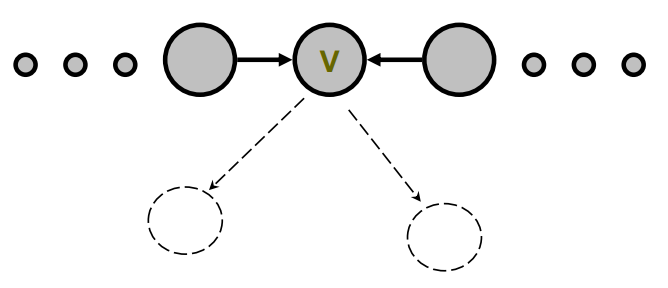
\includegraphics[width=0.35\textwidth]{./img/Reti/HeadToHead.png}
                  \caption{Collegamento head-to-head}
                  \label{fig:head-to-head}
              \end{figure}
    \end{itemize}
\end{definizione}
La d-separazione può essere calcolata in tempo lineare. Quindi abbiamo a
disposizione un algoritmo efficiente per inferire automaticamente se apprendere
il valore di una variabile può fornirci delle informazioni aggiuntive su altre
variabili, date le informazioni a disposizione.
\begin{teorema} [\textbf{Verma \& Pearl}]
    Se in una rete Bayesiana un insieme di variabili $E$ di evidenza D-separa
    $X$ e $Z$, allora $X$ e $Z$ sono indipendenti.
\end{teorema}
\begin{definizione}[\textbf{d-connessione}]
    Due variabili sono \textbf{d-connesse} se e solo se non sono d-separate.
\end{definizione}
Per testare se le variabili sono condizionalmente indipendenti si può usare il
Per testare se le variabili sono condizionalmente indipendenti si può usare il
\textbf{processo di moralizzazione}:
\begin{enumerate}
    \item \textbf{Disegnare grafo ancestrale}: rete composta delle variabili
          citate e tutti i loro predecessori.
    \item \textbf{Moralizzare il grafo}: per ogni coppia di variabili che hanno
          un figlio in comune, si traccia un arco non orientato tra di loro, in
          caso di più genitori si collegano le coppie a due a due.
    \item \textbf{Disorientiamo il grafo}: sostituzione degli archi orientati
          con archi non orientati
    \item \textbf{Eliminiamo i given e gli archi incidenti}: eliminare i nodi
          facenti parte dell'evidenza e tutte le connessioni.
\end{enumerate}
Se al termine di questo processo si hanno:
\begin{itemize}
    \item \textbf{Variabili disconnesse}: è garantito che le variabili sono
          indipendenti
    \item \textbf{Variabili connesse}: non è garantito che le variabili siano
          indipendenti.
\end{itemize}
\begin{esempio}
    Vediamo ora un esempio del processo di moralizzazione. Vogliamo verificare
    se $A$ e $B$ sono condizionalmente indipendenti dati $D$ e $F$.
    \begin{figure}[!ht]
        \centering
        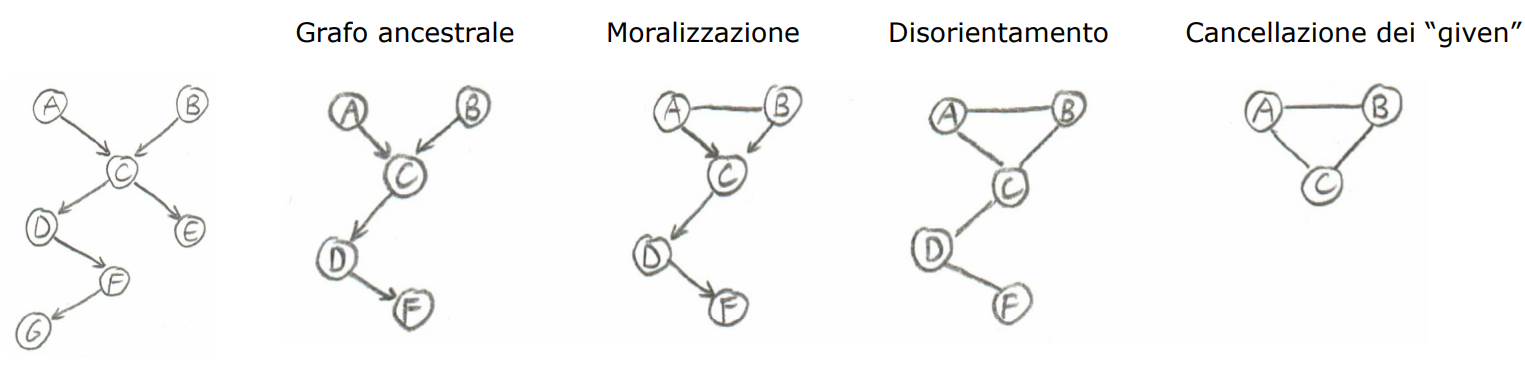
\includegraphics[width=1\textwidth]{./img/Reti/Moralizzazione.png}
        \caption{Esempio di moralizzazione}
        \label{fig:moralizzazione}
    \end{figure}
\end{esempio}
\subsection{Distribuzioni condizionali}
Per ridurre il numero di parametri nelle CPT possiamo utilizzare le \textbf{distribuzioni
    canoniche} per rappresentare dei pattern standard tra i parametri come per
i nodi deterministici. Si possono utilizzare le distribuzioni canoniche solo
quando si possono notare dei pattern particolari, ex: and tra genitori, or tra
genitori, somma dei genitori$\dots$

Una volta identificato il pattern, questo ci permette di specificare un numero
limitato di parametri per compilare la CPT, dal momento che alcuni si derivano
con le distribuzioni canoniche.
\begin{definizione}[\textbf{Nodo deterministico}]
    Un \textbf{nodo deterministico} è caratterizzato dal fatto che il valore che
    esso assume è completamente determinato tramite il valore assunto dai suoi
    genitori. Non c'è incertezza.
\end{definizione}
Le relazioni tra genitori e figli possono essere di diversi tipi:
\begin{itemize}
    \item \textbf{Logiche}: come ad esempio l'\texttt{OR} tra le variabili dei genitori.
    \item \textbf{Numeriche}: come ad esempio il \texttt{minimo} valore delle
          variabili dei genitori.
\end{itemize}
Un importante pattern è l'\textbf{indipendenza di uno specifico contesto} ovvero
quando la probabilità condizionata di un nodo è condizionalmente indipendente
da alcuni genitori dati certi valori di altri (if-else sintax).

Le relazioni incerte, possono essere caratterizzate dalle \textbf{Noisy Logical
    Relations} che permettono di modellare l'incertezza dei genitori nel causare
il figlio. Queste relazioni sono utili per modellare situazioni in cui la presenza
di un genitore non implica necessariamente la presenza del figlio.
Andiamo per esempio ad analizzare il modello \textbf{Noisy-OR}. Questo modello
consente di introdurre incertezza circa la capacità di ogni nodo genitore di
causare il valore vero della variabile figlio.

Il modello Noisy-OR effettua le seguenti ipotesi:
\begin{itemize}
    \item Tutte le possibili cause sono note
    \item L'inibizione di un genitore è indipendente dall'inibizione degli altri
          genitori per il nodo considerato.
\end{itemize}
In questo caso specifico la probabilità di un determinato evento, è data dal
prodotto delle probabilità di inibizione per ogni nodo genitore.
\subsection{Rappresentazioni efficiente delle distribuzioni continue}
Per rappresentare efficientemente i nodi di distribuzioni continue, usando quelle
canoniche, possiamo pensare di discretizzare le variabili continue definendo un
insieme finito di intervalli. Il problema che sorge utilizzando questo approccio
è legato alla perdita di informazioni sul dato. Inoltre, le CPT spesso aumentano
di dimensione.

Una soluzione alternativa è rappresentare le variabili con delle \textbf{funzioni
    di densità di probabilità} vengono descritte tramite un numero finito e di
norma contenuto di parametri. Un esempio è la funzione di densità di probabilità
della distribuzione normale, la quale viene completamente specificata tramite
la media e la deviazione standard.
\begin{definizione}[\textbf{Rete Bayesiana Ibrida}]
    Una rete che contiene nodi discreti e continui prende il nome di \textbf{Rete
        Bayesiane Ibrida}
\end{definizione}
Per specificare una Rete Bayesiana Ibrida dobbiamo definire due nuovi tipi di
distribuzione:
\begin{itemize}
    \item La distribuzione condizionale di una variabile continua dati i genitori
          discreti o continui.
    \item La distribuzione condizionale di una variabile discreta dati i genitori
          continui.
\end{itemize}
\section{Inferenza}
\subsection{Inferenza esatta}
Il compito primario di ogni sistema inferenziale probabilistico consiste nel
computare la distribuzione a posteriori, per un determinato insieme di \textbf{variabili
    di query}, quando si è osservato un determinato evento, ovvero un assegnamento
congiunto di valori per un insieme di \textbf{variabili di evidenza}.

In questa sezione useremo la seguente notazione:
\begin{itemize}
    \item $X$: la variabile di query.
    \item $E$: insieme di variabili di evidenza.
    \item $e$: specifico evento, ovvero un assegnamento congiunto dei singoli
          valori delle variabili di evidenza.
    \item $Y$: insieme di variabili non di evidenza.
\end{itemize}
L'insieme complessivo di variabili è rappresentato da:
\begin{equation*}
    V = \{X\} \cup E \cup Y
\end{equation*}
Una tipica query della quale bisogna calcolare la posterior è:
\begin{equation*}
    P(X|E=e)
\end{equation*}
Fino a questo momento, calcolavamo la distribuzione di probabilità di una
variabile date tutte le altre variabili nella rete.

Nelle reti bayesiane abbiamo diverse tipologia di inferenza:
\begin{itemize}
    \item \textbf{Diagnostica}: si passa dagli effetti alle cause, l'evidenza è
          nei discendenti e l'informazione sale dai figli ai genitori.
          \begin{figure}[!ht]
              \centering
              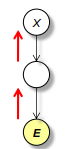
\includegraphics[width=0.08\textwidth]{./img/Reti/Diagnostica.png}
              \caption{Inferenza diagnostica}
              \label{fig:diagnostica}
          \end{figure}
    \item \textbf{Causale}: si passa dalle cause agli effetti, l'evidenza è
          nei genitori e l'informazione scende dai genitori ai figli.
          \begin{figure}[!ht]
              \centering
              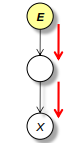
\includegraphics[width=0.08\textwidth]{./img/Reti/Causale.png}
              \caption{Inferenza causale}
              \label{fig:causale}
          \end{figure}
    \item \textbf{Intercausale}: si passa l'informazione tra le cause comuni
          a un effetto.
          \begin{figure}[!ht]
              \centering
              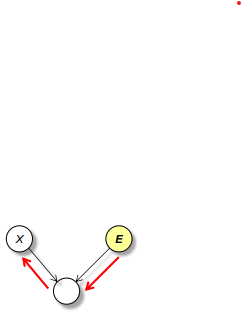
\includegraphics[width=0.2\textwidth]{./img/Reti/Intercausale.png}
              \caption{Inferenza intercausale}
              \label{fig:intercausale}
          \end{figure}
    \item \textbf{Mista}: combinazione di due o più delle tipologie di inferenza
          presentate in precedenza.
          \begin{figure}[!ht]
              \centering
              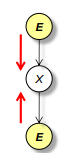
\includegraphics[width=0.08\textwidth]{./img/Reti/Mista.png}
              \caption{Inferenza mista}
              \label{fig:mista}
          \end{figure}
\end{itemize}
Conoscere l'evidenza di una variabile può influenzare la probabilità di altri nodi
nella rete. Quindi, quando si osserva un evento, si aggiornano le distribuzioni
di probabilità di tutti i nodi della rete. Una volta effettuato questa operazione,
è possibile eseguire le query sulle CPT aggiornate.

Per rispondere ad una query generica del tipo:
\begin{equation*}
    P(X|E=e)
\end{equation*}
allora posso sfruttare la seguente equazione, ovvero l'\textbf{algoritmo di
    enumerazione}:
\begin{equation}
    P(X|E = e) = \alpha P(X,E = e) = \alpha \sum_{y} P(X,E = e, Y = y)
\end{equation}
dove $\alpha$ mi rappresenta un parametro di normalizzazione, mentre $\sum_{y}
    P(X,E = e, Y = y)$ rappresenta la probabilità al variare delle variabili nascoste.

Si parla di enumerazione perché calcoliamo tutte le possibili combinazioni di valori
delle variabili che non fanno parte dell'evidenza.
\begin{nota}
    Si aggiunge la costante di normalizzazione, ovvero:
    \begin{equation}
        \alpha = \frac{1}{\sum_{x\in X}P(X = x)}
    \end{equation}
\end{nota}
Inoltre, possiamo sfruttare la regola di fattorizzazione per calcolare la probabilità
$P(X,E=e,Y=y)$, ovvero:
\begin{equation}
    P(X,E=e,Y=y) = \prod_{K} P(K=k | parents(K))
\end{equation}

In generale, quando si effettua l'inferenza in una rete Bayesiana, si calcola il
valore della variabile di query per tutti i suoi possibili assegnamenti:
\begin{equation*}
    P(X=x|E=e) = \langle P(X = x'|E = e), P(X = x''|E = e),\dots \rangle
\end{equation*}

Il processo di inferenza per $n$ variabili booleane è pari a $\mathcal{O}(n2^n)$.
Possiamo però migliorare le tempistiche attraverso delle semplificazioni:
\begin{itemize}
    \item Si può migliorare il calcolo $P(K=k | parents(K))$ andando a raccogliere
          i fattori che non dipendo dalle sommatorie. Così facendo si risparmiano
          delle moltiplicazioni.
    \item Dal momento che calcoliamo tutte le combinazioni dei valori delle
          variabili significa che alcuni valori vengono calcolati più volte.
          Quindi cambieremo approccio e useremo l'\textbf{algoritmo delle
              eliminazione delle variabili}.
\end{itemize}

L'algoritmo si basa sul principio di risolvere il calcolo delle sommatorie in
\textbf{bottom-up}, ovvero da destra verso sinistra e salvando i valori in modo
tale da calcolarlo senza ripetizione.
\subsection{Inferenza approssimata}
Permette di effettuare inferenza in tempi ragionevoli quando si hanno tante
variabili che non fanno parte dell'evidenza, infatti questo evita di ricadere
nell'NP-Hard con l'inferenza esatta. L'inferenza approssimata consiste nel
approssimare queste variabili libere, campionandole attraverso la generazione dei
numeri casuali.

In questo modo non si controllano le probabilità di tutte le combinazioni di valori
(i famosi $2^n$) ma si controllano le probabilità di una successione finita di
numeri casuali, non entrando nella complessità esponenziale.
Per valutare la complessità di un algoritmo di inferenza è importante considerare
la struttura della rete. Possiamo avere una rete con una struttura (vedi figura \ref{fig:struttura_reti}):
\begin{itemize}
    \item \textbf{Rete singolarmente connessa} (\textbf{Polytree}): dove si ha al
          massimo un cammino non orientato tra due nodi.
    \item \textbf{Rete Multiplamente connessa}: dove si hanno più cammini non
          orientati tra due nodi.
\end{itemize}

\begin{figure}[!h]
    \centering
    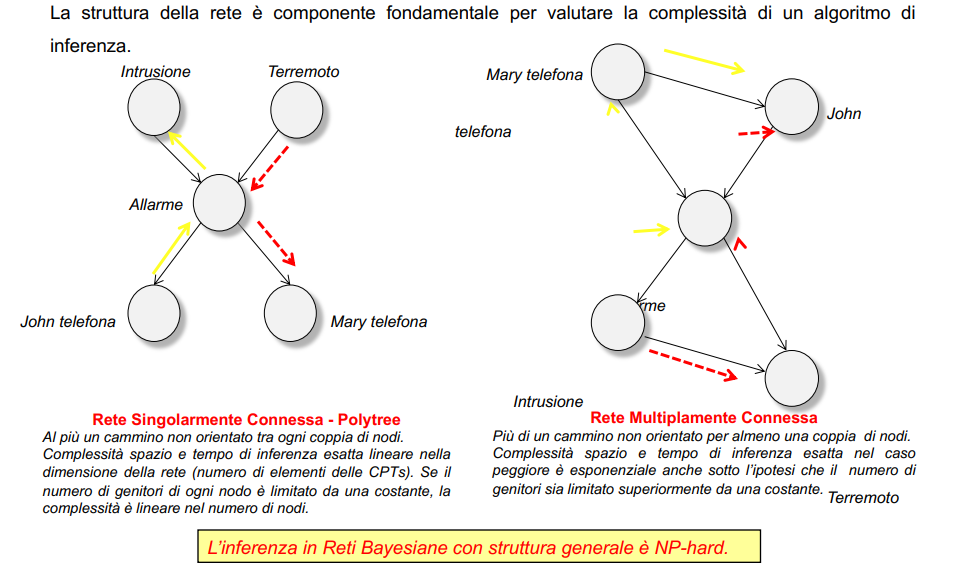
\includegraphics[width=0.8\textwidth]{img/Reti/struttura_reti_bayesiane.png}
    \caption{Esempio di struttura delle reti bayesiane}
    \label{fig:struttura_reti}
\end{figure}

Nella precedente sezione abbiamo visto l'algoritmo di eliminazione delle
variabili. Per calcolare l'inferenza approssimata l' Questo algoritmo, permette nel caso di una rete Polytree, di computare
la probabilità a posteriori per tutte le variabili richiede di effettuare $\mathcal{O}(n)$
query ognuna delle quali ha una complessità di $\mathcal{O}(n)$. Quindi l'algoritmo
ha una complessità di $\mathcal{O}(n^2)$.

L'impiego di un algoritmo appartenente alla classe degli \textbf{algoritmi di
    clustering} (join tree algorithms) consente di ridurre la complessità a $\mathcal{O}(n)$.

Il principio sul quale si basano questi algoritmi è rappresentato dal fatto di
unire i nodi di una rete formando clusters di variabili. Queste operazioni vengono
fatte per trasformare la rete in un Polytree nel quale applicare un algoritmo di
inferenza efficiente.

Resta comunque il problema che il problema di inferenza esatta è NP-Hard. Per
questo motivo introduciamo degli algoritmi di inferenza approssimata della categoria
\textbf{Monte Carlo}. L'accuratezza di questi metodi dipende dal numero di campionamenti
generati.
\subsubsection{Direct Sampling}
Questo metodo consiste nel campionare direttamente le variabili della rete ignorando
le evidenze. Il funzionamento di questo algoritmo si basa sull'ordinamento
topologico delle variabili della rete.

Nel dettaglio, il suo funzionamento è il seguente:
\begin{itemize}
    \item Si ordinano le variabili della rete in modo tale che ogni variabile
          sia preceduta dai suoi genitori.
    \item Partendo dalla prima variabile si genera un campione casuale sulla base
          della distribuzione espressa dalla CPT.
    \item Si prosegue con la generazione delle altre variabili tenendo in
          considerazione i valori delle variabili precedenti che sono già stati
          estratti.
    \item Si ripete questo procedimento per generare un numero finito di campioni.
\end{itemize}
Questo algoritmo genera campioni della distribuzione di probabilità congiunta a
priori per il modello di rete bayesiana specificata.

In ogni algoritmo di campionamento le risposte vengono computate tramite conteggio
dei campioni generati.

Questo metodo mi permette di generare campioni senza considerare le evidenze. Nel
caso in cui si voglia considerare le evidenze, si utilizza il metodo di \textbf{Rejection
    Sampling}.

Questo algoritmo genera campioni della probabilità congiunta e successivamente
rifiuta i campioni che non soddisfano le evidenze. La stima viene fatta sui
campioni non rigettati.

Purtroppo, l'algoritmo di Rejection Sampling rifiuta troppi campioni ed il tasso
di rigetto cresce esponenzialmente con il numero di variabili per le quali è
disponibile evidenza.

Questa particolarità rende sostanzialmente inutilizzabile l'algoritmo in questione
nel caso di modelli reali di Reti Bayesiane.
\subsubsection{Likelihood Weighting}
Questo algoritmo evita di generare campioni che dovranno essere successivamente
rigettati. Per fare questo fissa il valore dei nodi per i quali è disponibile
l'evidenza e genera i valori dei nodi rimanenti.

Inoltre, questo algoritmo pesa in modo differente i vari eventi, il peso di ogni
evento rappresenta la likelihood che l'evento associa all'evidenza.

Intuitivamente gli eventi per i quali l'evidenza disponibile è inverosimile devono
pesare in misura minore nel processo di stima delle probabilità a posteriori.

Campionare significa generare una serie di campioni:
\begin{equation*}
    s_i = \left[V_1=v_1, V_2= v_2, \dots, V_n=v_n\right]
\end{equation*}
dove $V_j$ sono tutte le variabili. Quando si eseque il processo di campionamento, 
se le variabili hanno evidenza, allora il loro valore nel campione è definito da essa.
Nel caso in cui non ci sia evidenza, allora si campiona la variabile secondo la
distribuzione data dalla CPT considerando le eventuali evidenze.

Questo rende importante rispettare l'ordinamento topologico quando si applica 
l'algoritmo di Likelihood Weighting.

Per ogni campione si ottiene un peso $\omega_i$, inizialmente posto a $1$, il 
quale viene aggiornato durante il campionamento sfruttando le probabilità dell'evidenza.
\begin{equation*}
    \omega_i = \omega_i \cdot P(E = e | Parents(E)
\end{equation*}
dove $E$ è una delle variabili di evidenza e $P(E=e | Parents(E))$ rappresenta la
probabilità di $E$ dato il valore dei genitori di $E$.

A questo punto per eseguire le query si calcola la probabilità valutando i pesi:
\begin{equation*}
    P(X = x | E = e) = \frac{\sum_{s_i, X=x} \omega_i}{\sum_{s_i} \omega_i}
\end{equation*}
\subsubsection{Markov Chain Monte Carlo (MCMC)}
Differentemente dagli algoritmi precedenti, i quali generano ogni evento partendo
da zero (si dimentica il campione precedente), l'algoritmo \textbf{Markov Chain Monte Carlo} 
genera ogni evento tramite modifiche casuali di un evento che lo precede nell'esecuzione.

È utile pensare che il modello di rete bayesiana si trovi in un determinato
\textbf{stato corrente}, il quale è identificato tramite l'assegnamento di un
valore ad ogni nodo della rete.

Lo stato prossimo viene ottenuto tramite campionamento di una delle variabili
senza evidenza $X_i$, si sceglie casualmente la variabile da campionare e si 
cambia il suo valore secondo la distribuzione condizionale della sua Markov Blanket.

Per generare lo stato successivo, parto dallo stato corrente, per ogni $X_i \not \in E$
(non nell'evidenza) cambio il suo valore estraendo un campione di $X_i$ secondo 
la distribuzione $P(X_i | MarkovBlanket(X_i))$. Alla fine avrò generato casualmente 
un nuovo campione.

Il calcolo di $P(X_i | MarkovBlanket(X_i))$ si effettua in questo modo:
\begin{equation}
    P(X_i | MarkovBlanket(X_i)) = \alpha \cdot P(X_i | parents(X_i)) \cdot 
    \prod_{Y_i\in children(X_i)} P(Y_i| parents(Y_i))
\end{equation}
\section{Generazione di numeri pseudocasuali}
\begin{definizione} [\textbf{Sequenza di numeri casuali}]
    Una \textbf{sequenza di numeri casuali} è una sequenza di realizzazioni di
    variabili aleatorie indipendenti e identicamente distribuite.
\end{definizione}
\begin{definizione} [\textbf{Sequenza di numeri pseudocasuali}]
    Una \textbf{sequenza di numeri pseudocasuali} è una sequenza di numeri che
    sembrano impredicibili da cui non si riesce ad estrarre alcuna regolarità.
\end{definizione}
Quindi i numeri casuali non sono regolati da una particolare regola, al contrario,
i numeri pseudocasuali hanno delle regolarità e si ripetono con un pattern.
\begin{nota}
    I metodi di generazione di numeri pseudocasuali implementati nei computer
    sono tutti basati sull'aritmetica.
\end{nota}
I numeri pseudocasuali devono soddisfare alcune proprietà:
\begin{itemize}
    \item \textbf{Indipendenza statistica}: tutti i numeri della sequenza devono
          essere indipendenti tra di loro.
    \item \textbf{Uniformità della distribuzione}: tutti i numeri della sequenza
          devono essere estratti dalla stessa distribuzione.
    \item \textbf{Riproducibilità della sequenza di valori}.
    \item \textbf{Non ripetitività su un prefissato periodo}: la sequenza non si
          deve ripetere in un dato periodo.
\end{itemize}
Una routine di generazioni di numeri pseudocasuali deve:
\begin{itemize}
    \item essere veloce
    \item avere un ciclo periodico sufficientemente lungo
    \item non presentare larghi gap
    \item essere replicabile
    \item generare numeri con proprietà statistiche simili a quelle ideali
\end{itemize}
\subsection{Generazione di numeri pseudocasuale}
\subsubsection{Metodo Naive}
Un primo metodo per generare numeri casuali è attraverso l'utilizzo di una sequenza
di numeri con $10$ cifre. Il procedimento è il seguente:
\begin{itemize}
    \item Si parte da un numero.
    \item Lo si eleva al quadrato.
    \item Si prendono le $10$ cifre centrali.
    \item Si ripete il procedimento.
\end{itemize}
La sequenza ottenuta \textbf{non è casuale}, perché ogni numero è ottenibile da
quello precedente. Inoltre, si hanno problemi a causa dell'operazione di elevamento
al quadrato, infatti si ha un'esplosione dei numeri.
\begin{esempio}
    Ecco un esempio di un problema su un numero a $4$ cifre.
    \begin{equation*}
        \begin{array}[pos]{cc}
            (6100)^2 & = 37\underline{2100}00 \\
            (2100)^2 & = 4\underline{4100}00  \\
            (4100)^2 & = 16\underline{8100}00 \\
            \vdots
        \end{array}
    \end{equation*}
\end{esempio}
\subsubsection{Moltiplicative Congruential Method (MCM)}
Sia $x_0$ il valore iniziale, o anche detto \textbf{seed}, della sequenza. Allora
un generico numero pseudocasuale può essere ottenuto da quello precedente nel
seguente modo:
\begin{equation}
    x_n = a \cdot x_{n-1} \mod M \quad 0 \leq x_n \leq M
\end{equation}
Con $a, M \in \mathbb{N}^+$.

Il problema di questo metodo è che genera sempre dei numeri in modo ciclico sulla
base del valore di $M$. Questo problema si può risolvere scegliendo opportunamente
il valore di $M$, solitamente si sceglie un valore molto grande e primo.
\subsubsection{Linear Moltiplicative Congruential Method (LCM)}
Questo metodo è una versione raffinata di quello precedente. In particolare, si
aggiunge un bias $c$, in modo tale da personalizzare la sequenza. In formule:
\begin{equation}
    x_n = (a \cdot x_{n-1} + c) \mod M
\end{equation}
dove $a,c,M \in \mathbb{N}^+$, inoltre $M > x_0, c, a$.

In ogni caso, a causa dell'operatore $\mod$, abbiamo sempre una periodicità dovuta
a $M$, quindi si cerca di scegliere tale valore in modo tale che sia grande e primo.
% TODO: chiedi al prof
\subsection{Generazione di una distribuzione generica}
Vogliamo avere degli approcci per generare casualmente dei numeri che rispettino
una distribuzione generica.

Per ottenere questo risultato, si utilizzano diversi metodi che a partire da un
numero random, estratto in modo uniforme tra $0$ e $1$, generano numeri che rispettano
una particolare distribuzione. Questi metodi sono:
\begin{itemize}
    \item \textbf{Trasformazione inversa}
    \item \textbf{Accettazione/rifiuto}
    \item \textbf{Composizione}
\end{itemize}
In sostanza si stanno generando variabili aleatorie.
\subsubsection{Trasformazione inversa}
Vogliamo generare una variabile aleatoria $X = x$ con una certa distribuzione.
Si parte dalla sua \textbf{funzione di probabilità} ($f_X(x)$) scelta, si ricava
la \textbf{funzione di probabilità cumulativa} ($F(X = x)$), quest'ultima funzione è:
\begin{itemize}
    \item continua
    \item monotona
    \item crescente
    \item limitata, compresa tra $[0,1]$
    \item definita nel seguente modo $F(X=x) =P(X \leq x) = \int_{-\infty}^X f_X(\tau) d\tau$
\end{itemize}
La generazione si effettua in questo modo:
\begin{itemize}
    \item Si seleziona la distribuzione che desideriamo per la variabile $X$,
          definendo $f_X(x)$ e successivamente $F(X=x)$.
    \item Si genera un numero $\mu \sim U([0,1])$.
    \item Si ottiene il numero randomico derivante dalla distribuzione di $X$
          nel seguente modo $x = F^{-1}(X=u)$.
\end{itemize}
Questo procedimento vale sia per variabili continue, sia per variabili discrete,
in questo caso la funzione di probabilità cumulativa è definita sostituendo una
sommatoria all'integrale.

Questo approccio coincide col campionamento della variabile $X$.
\begin{esempio}
    Sia $X$ la nostra variabile con $3$ simboli.
    \begin{equation*}
        P(X = x_0) = 0.1, \space P(X = x_1) = 0.3, \space P(X = x_2) = 0.6,
        F(X = x_i) = \sum_{l=0}^{i} P(X = x_l)
    \end{equation*}
    Sia $F^{-1}$ la funzione inversa della funzione cumulativa. Allora posso
    campionare tante volte la variabile $X$, generando tanti numeri casuali
    $\mu_i \in U([0-1])$.

    Sia $\mu_i = 0.2$ allora calcolo $F^{-1}(\mu_i) = x_1$ e allora genero $x_1$.
\end{esempio}
Il problema di questo approccio è che non sempre è possibile calcolare $F^{-1}$ o
spesso è complesso.
\subsubsection{Acceptance rejection}
Si può utilizzare per generare numeri $x$ derivanti da distribuzioni $X$ limitate
da intervalli finiti $[a,b]$.

Scegliendo una distribuzione $f_X$ per a variabile aleatoria $X$ tale che sia
definita solo in $[a,b]$ e quindi:
\begin{equation}
    f_X : [a,b] \rightarrow [0,c]
\end{equation}
\begin{osservazione}
    In pratica la funzione $f_X$ è tutta contenuta all'interno del rettangolo
    $[a,b] \times [0,c]$.
\end{osservazione}
\begin{figure}[!ht]
    \centering
    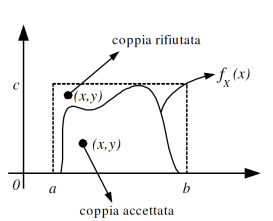
\includegraphics[width=0.3\textwidth]{./img/Reti/acceptancerejection.png}
    \caption{Acceptance rejection}
    \label{fig:acceptance-rejection}
\end{figure}
Il metodo si basa sul generare coppie di numeri $\mu_i,\mu_j$ estratti da due
sequenze pseudocasuali estratte da distribuzioni $U[0, 1]$. Da queste, genereremo
due sequenze di numeri utilizzando:
\begin{equation}
    \begin{cases}
        x = a + (b-a)\mu_i \\
        y = cf_X(x)\mu_j
    \end{cases}
\end{equation}
se la coppia $(x_i, y_i)$ cade all'interno dell'area sottesa alla curva della
funzione $f_X(x)$ allora sarà accettata e verrà utilizzata per generare la sequenza
di numeri casuali, altrimenti viene rigettata e si ripetono i passi fino a quando
non troviamo una coppia ammessa.